%!TEX TS-program = xelatex
%!TEX encoding = UTF-8 Unicode
% Awesome CV LaTeX Template for CV/Resume
\documentclass[a4paper,12pt]{awesome}

\usepackage{graphicx}
\graphicspath{ {./images/} }

\fontdir[fonts/]
%-----------------------------------------------------------
\usepackage[top=0.3in, bottom=0.5in, left=0.5in, right=0.5in]{geometry}

\usepackage{url}
\usepackage{palatino}
\usepackage{tabularx}
\usepackage{hyperref}
\usepackage{color}
\hypersetup{
    colorlinks=true,
    linkcolor=blue, 
    urlcolor=blue,
}

\setlength{\tabcolsep}{0in}
\newcommand{\isep}{-2 pt}
\newcommand{\lsep}{-0.5cm}
\newcommand{\psep}{-0.6cm}

\begin{document}
\ \linebreak
\headerfirstnamestyle{DILIP }\headerlastnamestyle{SHARMA} \hfill Email-id : \entrytitlestyle{2017csb1073@iitrpr.ac.in} \linebreak
\headersocialstyle{B.Tech. In Computer Science And Engineering} \hfill Mobile No.: \entrytitlestyle{+91-8896740277} \linebreak
\headersocialstyle{Indian Institute of Technology, Ropar} \hfill Github : \href{https://github.com/dilip640}{dilip640}
\linebreak \linebreak
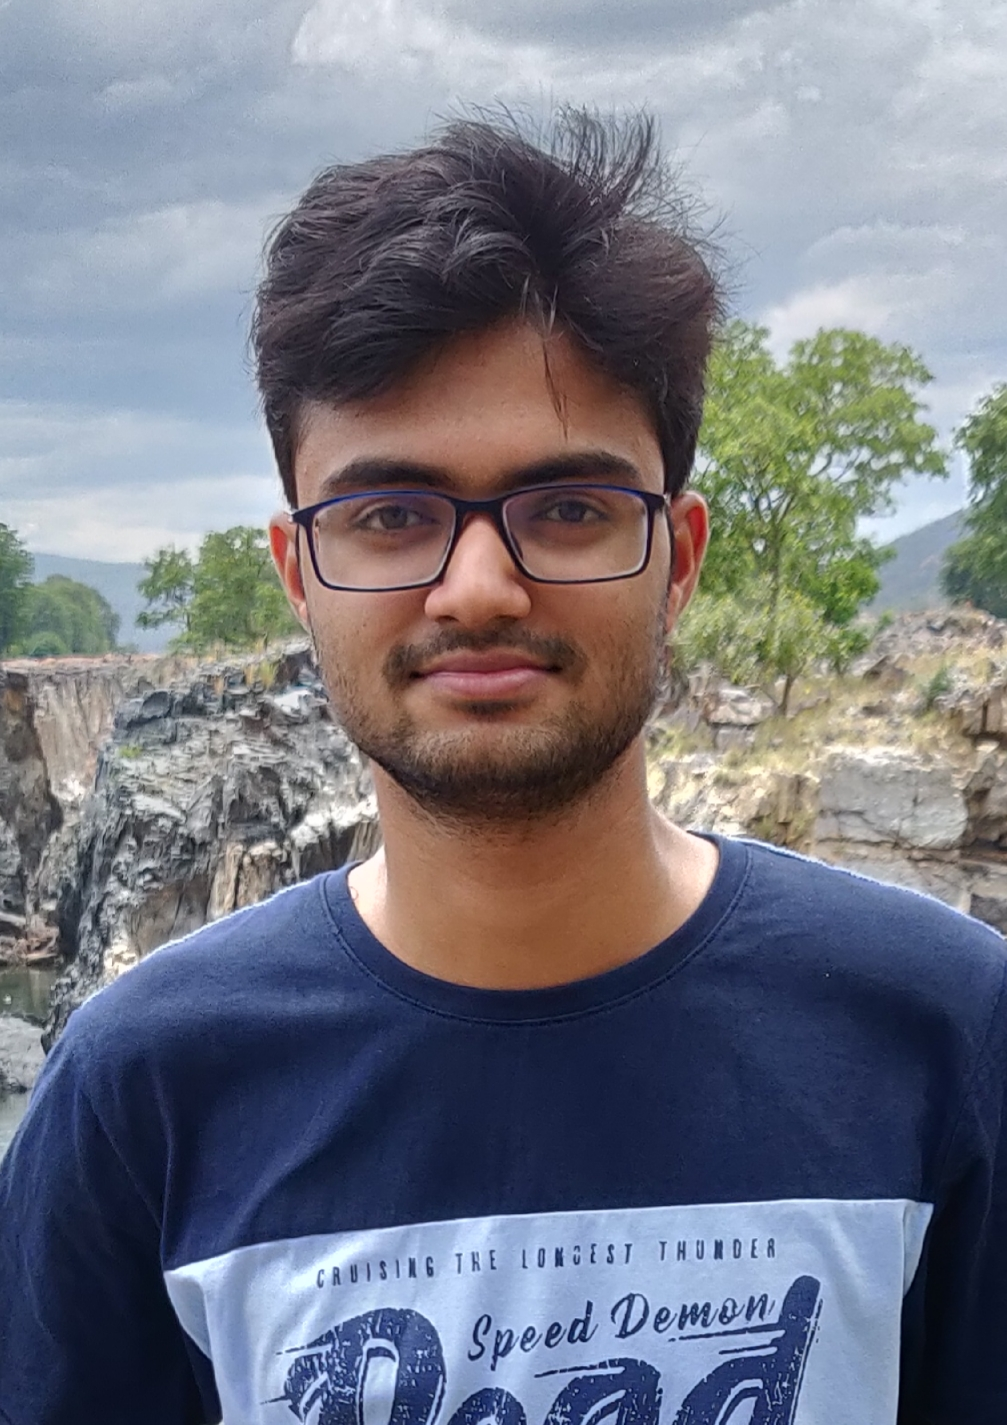
\includegraphics[width=4cm, height=5cm]{dilip-sharma}
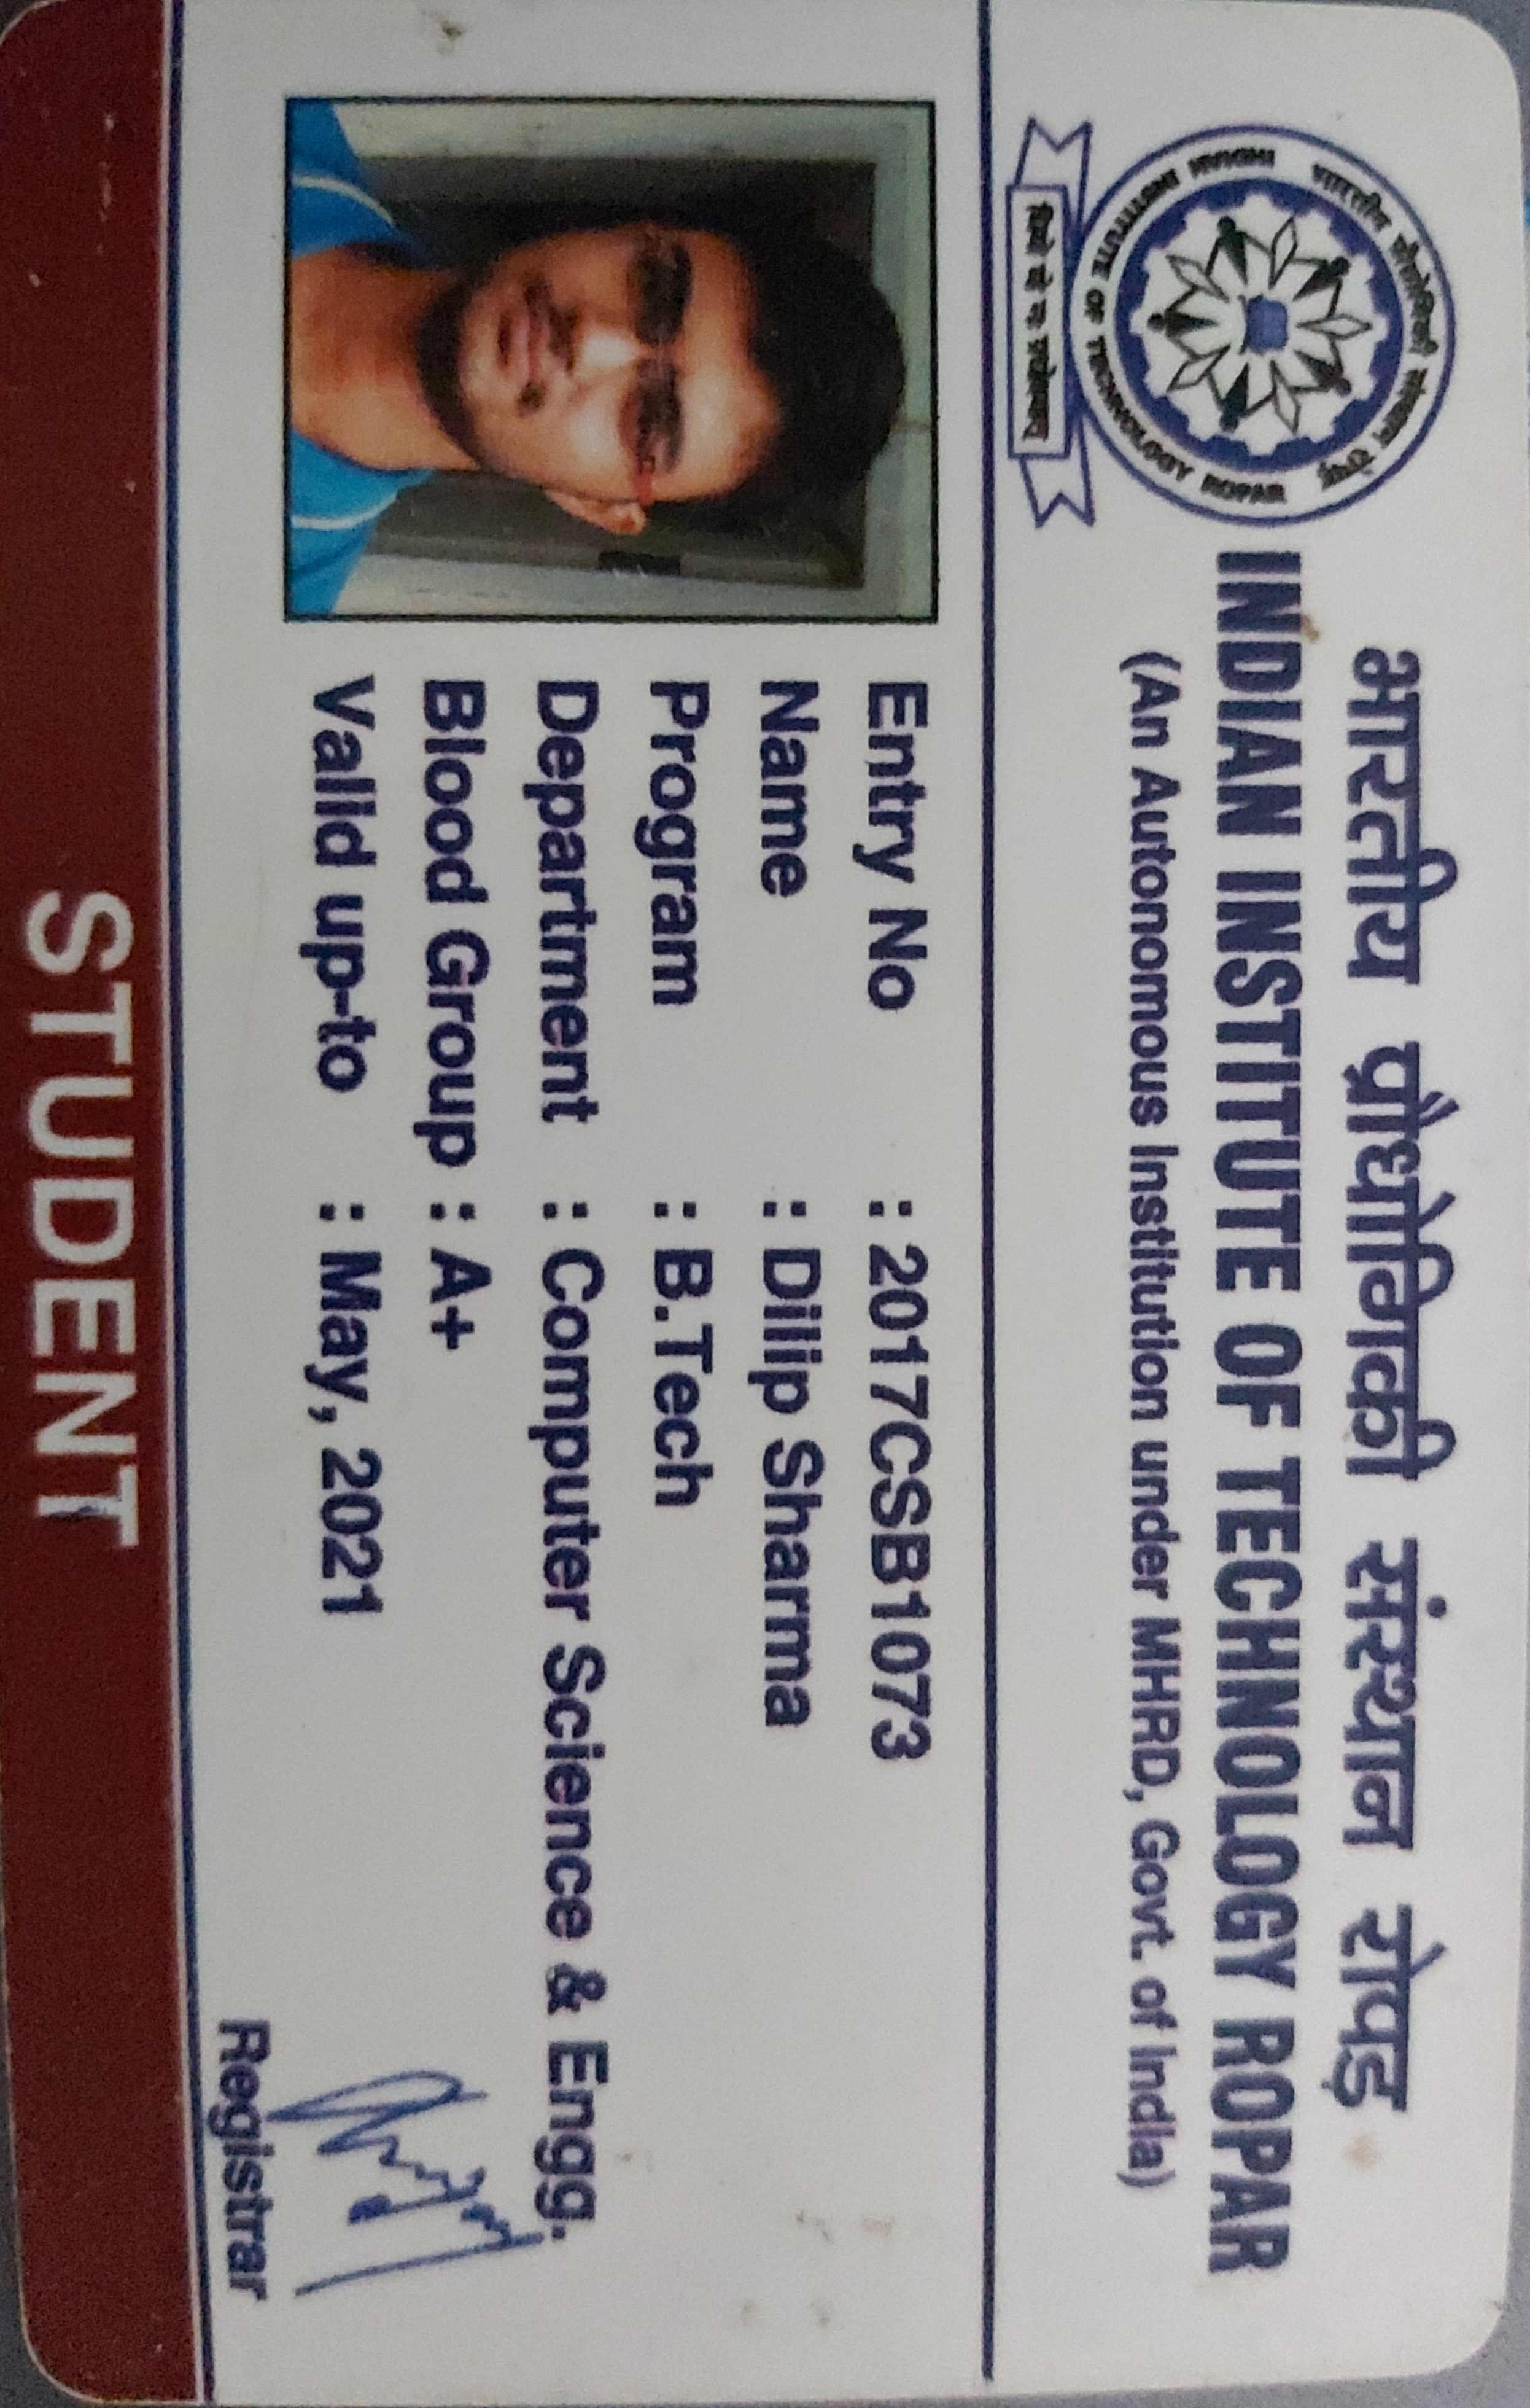
\includegraphics[width=10cm, height=5cm]{institute-id}
\linebreak

\cvsection{ACADEMIC DETAILS}

\begin{tabular}{ l @{\hskip 0.12in} l @{\hskip 0.12in} l @{\hskip 0.12in} l @{\hskip 0.12in} l }

\textbf{Qualification} & \textbf{University} & \textbf{Institute} & \textbf{Year} & \textbf{CGPA/Aggregate\%} \\

B.Tech.& IIT Ropar & IIT Ropar  - India & 2017-Present & 6.97/10 \\
Intermediate :& BSEB & R S +2 High School Adhaura, Bhabua & 2016  &  72\% \\
Matriculation :& CBSE & Universal Public School Baburi, Chandauli  & 2014& 9.2/10 \\
\end{tabular} \linebreak
\cvsection{SKILLS}\linebreak
\indent 
\begin{tabular}{ l @{\hskip 0.006cm} l }
    \textbf{Programmings Languages } & C/C++, Go, Python, JAVA, HTML5, CSS, PHP, JavaScript \\
    \textbf{Frameworks / Libraries} & Tensorflow, Beam, Qor, OpenCV, Flutter, Django, Angular \\ 
    \textbf{Software / Tools / OS} & Dataflow, Kubeflow, Kubernetes, HAProxy, Prometheus, Git, Android Studio  \\
\end{tabular}\\
\linebreak
\cvsection{WORK EXPERIENCE}\\[\psep]
\begin{enumerate}
\item[] Data Science Intern, \textbf{\href{https://www.xlpat.com}{XLPAT}}\\
    \emph{(WFH Internship, April-October(Expected) 2020)} \hfill  \emph{Xlpat Labs Mohali}\\[-0.6cm]
    \begin{itemize}
        \item Implemented \textbf{Zero-Shot Learning} for auto-categorize patents based on user input categories and trained model on
         massive patents data from Google Bigquery.
        \item Trained \href{https://github.com/src-d/tensorflow-swivel}{Swivel} Word Embedding on a vast text corpus of 200GB using MultiWorkerMirroredStrategy with TFjob.
        \item Skills learned: Tensorflow, Kubeflow Pipeline, Tfjob, Apache Beam, Dataflow Runner
    \end{itemize}
\item[] Product Engineering Intern, \textbf{\href{https://www.gojek.io/}{Gojek}}\\
    \emph{(Summer Internship, May-July 2019)} \hfill  \emph{Gojek Tech Bangalore}\\[-0.6cm]
    \begin{itemize}
        \item Built a system \textbf{Hospital}, which fixes known failures for a system 
            automatically by a given run-book
        \item Skills learned: System Design, Golang, Unit Testing, Load Balancer, Polling, 
            Containerization, CI/CD, Monitoring System
        \item The project is open-sourced at \href{https://github.com/gojekfarm/hospital}{gojekfarm/hospital}.
    \end{itemize}
\end{enumerate}
\cvsection{PROJECTS}\\[\psep]
\begin{enumerate}
    \item \textbf{Electronic Invoicing using Image Processing}
        \hfill \emph{Flipkart Grid Challenge, July '20}\\[-0.6cm]
        \begin{itemize}
            \item Built a digital platform for automatically digitizing physical invoices. 
            Microservices architecture was used for scalability
            \item Novel approach of extracting Key-Value pairs and Table separately using
            Deep Learning model was used; ML model gave good results on any general template of Invoice
            \item Used \textbf{FastAPI} for async support required for ML tasks; \textbf{gRPC} for internal communications 
            and published all services on \textbf{Docker Hub} for deployment; Clova AI was used for OCR. 
            (\href{https://docs.google.com/document/d/1X1sg_pPHy_magULwscUbH0_RvUvilRWutCnh3Fi92Cc/view}{Source code})
        \end{itemize}
    \item \textbf{RISC-V Assembly Language Simulator}
        \hfill \emph{March-April 19, Python}\\[-0.6cm]
        \begin{itemize}
            \item Built a 32bit RISC-V Assembly language simulator with 5 stages instruction execution 
                with pipelining and also implemented Cache level memory system
            \item Used PyQT to make GUI like \href{http://www.kvakil.me/venus/}{Venus}, 
                a simulator for RISC-V. (Source code: \href{https://github.com/dilip640/RISC-V-Simulator}{Github})
        \end{itemize}
    \item \textbf{Classification of Mail into Ham/Spam}
        \hfill  \emph{ Jan 18, Python/C} \\[-0.6cm]
        \begin{itemize}
            \item Used K-Means Clustering Algorithm on input files to classify messages into ham/spam
            \item Also used Naive-Bayes Classification for the same purpose
            \item Naive-Bayes Classification's result was more accurate
        \end{itemize}
    \item \textbf{Published Android App to Play store}
    \hfill  \emph{Summer 2018, Android Studio, java} \\[-0.6cm]
    \begin{itemize}
        \item \textbf{2M+ Downloads} on Play Store (\href{https://play.google.com/store/apps/details?id=com.extricks.whatsdeleted}{link})
        \item Captures WhatsApp deleted messages from Notification Bar
	    \item Also Captures deleted Media files of WhatsApp
    \end{itemize}
    \item \textbf{Rectangle Detection using OpenCV}
    \hfill  \emph{Dec 2018, Android Studio, java} \\[-0.6cm]
    \begin{itemize}
       \item Made an android app which will capture photo and will search for a rectangle of appropriate size. 
	    \item Using tesseract API it extracts texts within the rectangle.
    \end{itemize}
\end{enumerate}
\cvsection{RELEVANT COURSES}\\[\lsep]
    \begin{itemize}
        \item \textbf{Computer Science: }Data Structures and Algorithms, Computer Architecture, Digital Logic Design, 
            Introduction to Computing and Data Structures, Programming Paradigms And Pragmatics,
            Computer Networks, Introduction to Database System, Operating Systems, Software Engineering,
            Theory of Computation
	    \item \textbf{Mathematics: }Probability and Statistics, Discrete Mathematics, Calculus, Linear Algebra, Differential Equations
    \end{itemize}
\cvsection{ACHIEVEMENTS AND RESPONSIBILITIES}\\[\lsep]
\begin{enumerate}\itemsep \isep
    \item Representative of Software Club IIT Ropar
    \item Core Member of Advitiya 2020 IIT Ropar Technical fest
    \item Participated in Hackathon of Advitiya'19 IIT Ropar Technical fest, 
        \headerquotestyle{Created an Android Application using Flutter for UI and Django as back-end where Artist can interact
        with Producer. List of Producers was recommended to the video uploaded by Artist. YOLO and The Random Forest
        machine learning algorithms were used for making the Recommendation Engine. 
        Link to code on \href{https://github.com/jainammm/Tropikat-advitiya}{Github}}
    \item Won Hackathon in Quintessence’18, Intra-College Technical fest, \headerquotestyle{Created an Android 
        Application using which creates a buyer-seller System.
        It gives the buyer the nearest seller of his required item. Firebase platform was used 
        for creating database and login system. Link to code on 
        \href{https://github.com/dilip640/Daiquiris}{Github}}
    \item Participated in Annual Sports Fest of IIT-BHU
\end{enumerate}
\end{document}